\chapter{Key Decisions and Outline of Trading Strategies}

\section{Liquidity Pools} \label{sec:liquidity-pools}
As previously mentioned, Uniswap is a decentralized exchange protocol that facilitates swapping of cryptocurrencies through the use of liquidity pools. One of the remarkable features of Uniswap is its support for even the smallest cryptocurrencies. In fact, it currently possesses 12,182 liquidity pools, as obtained via the Uniswap V3 subgraph. The subgraph provides valuable insights into the liquidity pools within the Uniswap ecosystem.
\\[5mm]
Table \ref{tab:liquidity_pools} showcases the diversity of these pools. Some pools exhibit high trading volumes, indicating significant activity and demand for those specific pairs. On the other hand, there are also pools with zero liquidity, which could be attributed to various reasons. It could be due to a lack of demand for one of the token pairs offered in the pool, or it may indicate that the pool is relatively new and has not attracted significant participation yet.
\\[5mm]
To enhance the chances of successful swaps and maximize potential profitability, my strategy is centered on liquidity pools with a trading volume surpassing \$10,000,000 (or \$10 million) and pools that include tokens supported by AAVE. Additionally, I exclude any liquidity pools that do not involve WETH, which is a tokenized form of ETH (Ethereum's native cryptocurrency). WETH's key advantage lies in its ability to align with ERC-20 standards, enabling broader compatibility and utilization across the Ethereum ecosystem.

\begin{table}[!ht]
    \centering
    \begin{tabular}{|p{7em}|p{4em}|p{4em}|p{10em}|p{\linewidth / 6}|p{4em}|}
    \hline
        pool address & token0 & token1 & volume in USD & created at timestamp & feetier \\ \hline
        \truncate{7em}{0x88e6a0c2ddd26feeb64f039a2c41296fcb3f5640} & USDC & WETH & \truncate{10em}{375230561243.465} & 1620250931 & 500 \\ \hline
        \truncate{7em}{0x8ad599c3a0ff1de082011efddc58f1908eb6e6d8} & USDC & WETH & \truncate{10em}{70454095868.0967} & 1620169800 & 3000 \\ \hline
        \truncate{7em}{0x11b815efb8f581194ae79006d24e0d814b7697f6} & WETH & USDT & \truncate{10em}{62385006691.8387} & 1620251172 & 500 \\ \hline
        \truncate{7em}{0x3416cf6c708da44db2624d63ea0aaef7113527c6} & USDC & USDT & \truncate{10em}{57192593471.8346} & 1636825557 & 100 \\ \hline
        \truncate{7em}{0x4585fe77225b41b697c938b018e2ac67ac5a20c0} & WBTC & WETH & \truncate{10em}{49170385539.9928} & 1620246230 & 500 \\ \hline
        \truncate{7em}{0x4e68ccd3e89f51c3074ca5072bbac773960dfa36} & WETH & USDT & \truncate{10em}{30135014933.0963} & 1620232628 & 3000 \\ \hline
        \truncate{7em}{0x60594a405d53811d3bc4766596efd80fd545a270} & DAI & WETH & \truncate{10em}{26075053939.434} & 1620237823 & 500 \\ \hline
        \truncate{7em}{0xcbcdf9626bc03e24f779434178a73a0b4bad62ed} & WBTC & WETH & \truncate{10em}{21870989841.1326} & 1620158974 & 3000 \\ \hline
        \truncate{7em}{0x5777d92f208679db4b9778590fa3cab3ac9e2168} & DAI & USDC & \truncate{10em}{16143305036.8948} & 1636771503 & 100 \\ \hline
        \truncate{7em}{0x7858e59e0c01ea06df3af3d20ac7b0003275d4bf} & USDC & USDT & \truncate{10em}{15473402409.0591} & 1620159478 & 500 \\ \hline
        \truncate{7em}{0x99ac8ca7087fa4a2a1fb6357269965a2014abc35} & WBTC & USDC & \truncate{10em}{12568187132.1649} & 1620241995 & 3000 \\ \hline
        \truncate{7em}{0xc2e9f25be6257c210d7adf0d4cd6e3e881ba25f8} & DAI & WETH & \truncate{10em}{12519316091.9979} & 1620159368 & 3000 \\ \hline
        \truncate{7em}{0xe0554a476a092703abdb3ef35c80e0d76d32939f} & USDC & WETH & \truncate{10em}{9381529300.20357} & 1636926269 & 100 \\ \hline
        \truncate{7em}{0x6c6bc977e13df9b0de53b251522280bb72383700} & DAI & USDC & \truncate{10em}{7219493916.70291} & 1620158293 & 500 \\ \hline
        \truncate{7em}{0xac4b3dacb91461209ae9d41ec517c2b9cb1b7daf} & APE & WETH & \truncate{10em}{6621032721.87519} & 1647516735 & 3000 \\ \hline
        \truncate{7em}{0x8c54aa2a32a779e6f6fbea568ad85a19e0109c26} & FEI & USDC & \truncate{10em}{6206853090.73714} & 1621839430 & 500 \\ \hline\hline
        \truncate{7em}{0x53dd58b3143f428b449c16dd5706cee7d7bcf408} & sOHM & gOHM & 0 & 1652914688 & 10000 \\ \hline
        \truncate{7em}{0xbc90c4de85a4b559060cb28abfd4476ab6711f1a} & SHIB & NSTIC & 0 & 1652910391 & 100 \\ \hline
        \truncate{7em}{0xaa1297b08d0035f06309c1bfa36582c24b4ae361} & BUSD & DPC & 0 & 1674655715 & 100 \\ \hline
        \truncate{7em}{0x75087e5330c97f7ec7f716c6566f214cb0029f6a} & DAI & ICAP & 0 & 1652899566 & 10000 \\ \hline
        \truncate{7em}{0xc65a680191bd17a18c957c8aa2d1155ed2322792} & stkAAVE & FRAX & 0 & 1652817927 & 10000 \\ \hline
        \truncate{7em}{0x94589b18b95b355ee9a900f3df671b431779e20a} & VVV & SOL & 0 & 1674701603 & 10000 \\ \hline
        \truncate{7em}{0xf42f0def92337b6a83753c9fae6d579f7d67aaa9} & APEFI & ApeUSD & 0 & 1652808878 & 3000 \\ \hline
        \truncate{7em}{0xb9ba65f1568b318ffc1879a4a6368ef2b5ac96b8} & FRAX & ApeUSD & 0 & 1652808680 & 500 \\ \hline
        \truncate{7em}{0x1dfb167f1ba47f3bf835eb60a9317b4601925642} & GHD & WETH & 0 & 1652784327 & 3000 \\ \hline
    \end{tabular}
    \caption{A selection of liquidity pools on Uniswap \label{tab:liquidity_pools}}
\end{table}

\subsection{Correlated and Cointegrated Liquidity Pools}
Once the liquidity pools of interested in have been identified, it is crucial to filter the pool pairs based on their correlation. This is because correlated pairs tend to exhibit similar pricing movements thus would be possible to apply the mean reversion trading strategies. However, it is important to strike a balance between a highly correlated pair and a low correlated pair, as excessively high correlation can result in minimal price deviations, leading to fees that exceed the deviations and resulting in overall losses instead of profits. To address this, I have set a condition where the correlation coefficient ($\rho$) should fall within the range of $0.990 \leq \rho \leq 0.997$.
\\[5mm]
To determine which liquidity pools are cointegrated, I employed the Engle-Granger approach. The Engle-Granger test for cointegration involves several steps. Firstly, a unit root test is performed individually on each time series using methods like the Augmented Dickey-Fuller (ADF) test or the Phillips-Perron (PP) test. These tests assess whether the time series are stationary or exhibit unit roots (non-stationary) individually. For cointegration to hold, both time series must be non-stationary.
\\[5mm]
Once it is established that both time series are non-stationary, an estimation of the cointegration equation is derived. Typically, a linear regression model is employed to capture the long-term relationship between the time series variables. This equation provides an understanding of how the variables are linked over a long period.
\\[5mm]
Subsequently, a unit root test is conducted on the residuals obtained from the regression analysis. If the residuals are stationary (indicating the absence of unit roots), it suggests the presence of cointegration between the time series. This implies that the variables move together in the long run, even if short-term deviations occur.
\\[5mm]
By following the aforementioned sequence of steps in the Engle-Granger test, it enables us to determine which liquidity pools demonstrate cointegration, thereby emphasizing their interconnectedness and mutual relationship over time. The outcome of the cointegration tests for all possible combinations of liquidity pools is presented in Table \ref{tab:coin_pools}. This table provides a comprehensive list of the liquidity pool pairs along with the results of their respective cointegration tests and the correlation coefficient of each combination.
\begin{table}[!ht]
    \centering
    \begin{adjustwidth}{-1in}{-0.9in}
        \begin{tabular}{|p{12em}|p{12em}|p{5em}|p{4.2em}|p{4.2em}|p{4.2em}|p{3.5em}|}\hline
            pool1 & pool2 & t-statistic of unit-root test on residuals & \multicolumn{3}{|c|}{Critical Values} & Corr Coeff\\[-1ex]\cline{4-6}
            &   &   & 1\% & 5\% & 10\% & \\\hline
            \truncate{12em}{USDC\_WETH\_0x88e6a0c2ddd26feeb64f039a2c41296fcb3f5640} & \truncate{12em}{USDC\_WETH\_0xe0554a476a092703abdb3ef35c80e0d76d32939f} & -11.280314 & -3.898076 & -3.337043 & -3.045083 & 0.995244\\\hline
            \truncate{12em}{USDC\_WETH\_0x8ad599c3a0ff1de082011efddc58f1908eb6e6d8} & \truncate{12em}{USDC\_WETH\_0xe0554a476a092703abdb3ef35c80e0d76d32939f} & -11.183921 & -3.898089 & -3.33705 & -3.045089 & 0.995049\\\hline
            \truncate{12em}{WETH\_USDT\_0x11b815efb8f581194ae79006d24e0d814b7697f6} & \truncate{12em}{USDC\_WETH\_0xe0554a476a092703abdb3ef35c80e0d76d32939f} & -9.988616 & -3.898076 & -3.337043 & -3.045083 & 0.995075\\\hline
            \truncate{12em}{WETH\_USDT\_0x4e68ccd3e89f51c3074ca5072bbac773960dfa36} & \truncate{12em}{USDC\_WETH\_0xe0554a476a092703abdb3ef35c80e0d76d32939f} & -9.890807 & -3.898088 & -3.337049 & -3.045088 & 0.994951\\\hline
            \truncate{12em}{DAI\_WETH\_0x60594a405d53811d3bc4766596efd80fd545a270} & \truncate{12em}{USDC\_WETH\_0xe0554a476a092703abdb3ef35c80e0d76d32939f} & -11.369096 & -3.898076 & -3.337043 & -3.045083 & 0.995187\\\hline
            \truncate{12em}{DAI\_WETH\_0xc2e9f25be6257c210d7adf0d4cd6e3e881ba25f8} & \truncate{12em}{USDC\_WETH\_0xe0554a476a092703abdb3ef35c80e0d76d32939f} & -10.398429 & -3.898317 & -3.337177 & -3.045177 & 0.995004\\\hline
            \truncate{12em}{USDC\_WETH\_0xe0554a476a092703abdb3ef35c80e0d76d32939f} & \truncate{12em}{USDC\_WETH\_0x7bea39867e4169dbe237d55c8242a8f2fcdcc387} & -7.561677 & -3.901185 & -3.338775 & -3.046286 & 0.994488\\\hline
            \truncate{12em}{USDC\_WETH\_0xe0554a476a092703abdb3ef35c80e0d76d32939f} & \truncate{12em}{WETH\_USDT\_0xc5af84701f98fa483ece78af83f11b6c38aca71d} & -9.76086 & -3.90143 & -3.338911 & -3.04638 & 0.994551\\\hline
            \truncate{12em}{USDC\_WETH\_0xe0554a476a092703abdb3ef35c80e0d76d32939f} & \truncate{12em}{DAI\_WETH\_0xa80964c5bbd1a0e95777094420555fead1a26c1e} & -6.91588 & -3.905801 & -3.341344 & -3.048068 & 0.994107\\\hline
        \end{tabular}
    \end{adjustwidth}
    \caption{Cointegration test on Liquidity Pool pairs \label{tab:coin_pools}}
\end{table}

\noindent Based on the results obtained, we focus our further investigation solely on the pairs of liquidity pools that exhibit cointegration under a 1\% confidence level. This filtering process allows us to narrow down our analysis to those pairs where a long-term relationship exists, suggesting that they move together in a concerted manner.
\\[5mm]
By concentrating on the cointegrated pairs, we can delve deeper into exploring their dynamics, assessing their behavior, and leverage the interconnectedness between these liquidity pools. This approach enables us to prioritize our analysis and concentrate on the most relevant liquidity pool combinations that offer potential opportunities for profitable trading or other related activities.
 
\section{Strategy}

As previously mentioned, the strategy I employ is the mean reversion trading strategy. The basic concept of a mean reversion strategy identifying two closely related assets or securities, typically referred to as a pair, and taking advantage of deviations from their historical price relationship. This works by initially identifying a pair of assets that have a historically stable relationship as I have done in Section \ref{sec:liquidity-pools}. Then as prices change you calculate the spread, which is the difference between their prices. Look for deviations from the historical mean spread, upon a deviation one buys the undervalued asset and sells the other. The positions are then closed once the spread reverts back to its historical mean.

\subsection{Hedge Ratio}
In the mean reversion strategy, the hedge ratio refers to the ratio or proportion between the positions of two assets involved in a pairs trading strategy. It determines the optimal allocation of capital between the assets to minimize risk and create a market-neutral position. The hedge ratio represents the number of units or shares of one asset that should be held for each unit or share of the other asset in order to create a balanced or hedged position. It is derived through statistical techniques such as regression analysis.

\subsubsection{Mean Reversion Strategy}
In the simple mean reversion strategy, the approach relies on a given historical dataset, assuming that the hedge ratio between the paired assets remains consistent over the long term. To determine this hedge ratio, the Ordinary Least Squares (OLS) regression method is employed. In Python, the calculation can be carried out using the following steps:
\vspace{5mm}
\begin{lstlisting}[language=Python]
model = sm.OLS(history_p1, sm.add_constant(history_p2))
results = model.fit()
# Gradient of the OLS i.e. X = results.params[0] + results.params[1] * 'p2_token1_price'
hedge_ratio = params[1]
\end{lstlisting}
\vspace{5mm}
In Figure \ref{fig:f1}, the observed trend reveals that the gradient, representing the rate of change, exhibits a proximity to the value of 1. This indicates a relatively balanced relationship between the prices of each pair. However, it is important to note that as time progresses, any fluctuations or deviations from the exact value of 1 are minimal and have a negligible impact on the overall trend. The stability of the gradient over time suggests a consistent and relatively stable relationship between the liquidity pools, reinforcing the notion that their interdependence remains relatively constant.
\begin{figure}[!htb]
    \centering
    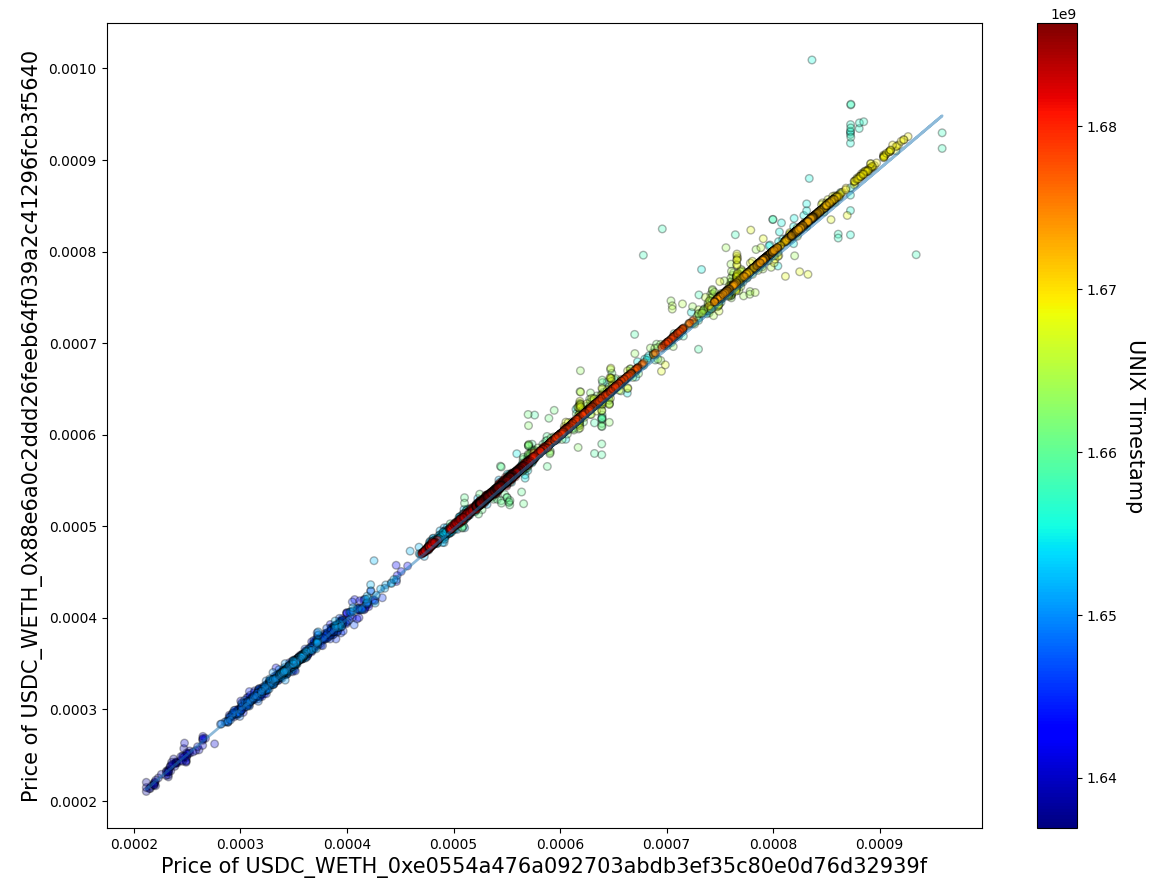
\includegraphics[width=0.8\textwidth]{project/Images/simple_hedge_ratio.png}
    \caption{Conducting OLS to obtain the Hedge Ratio \label{fig:f1}}
\end{figure}

\subsubsection{Kalman Filter}
As mentioned earlier, the hedge ratio plays a crucial role in minimizing risk and achieving a market-neutral position in trading strategies. However, relying on a fixed hedge ratio may not be ideal, as market dynamics and the relationship between the paired assets can change over time. To address this challenge, I employ the Kalman Filter as a dynamic tool to update and adapt the hedge ratio, taking into account the changing market conditions and the evolving relationship between the paired assets. This allows for a more responsive and adaptive approach to maintaining a market-neutral position. The Kalman Filter takes into consideration not only the current price data but also the historical information and the underlying dynamics of the assets. It provides a more robust and accurate estimation of the optimal hedge ratio, which aligns with the mean reversion strategy's objective of capturing potential price divergences and profiting from their eventual convergence.
\\[5mm]
The Kalman Filter works by iteratively updating and refining its estimate of the system state using a prediction step and an update step. For this an initial `guess' of the parameters that I use is the using the Ordinary Least Squares from the historical information provided. The remainder of the parameters that are selected can be seen below:
\vspace{5mm}
\begin{lstlisting}[language=Python]
model = sm.OLS(price_history_2, sm.add_constant(price_history_1))
initial_state = model.fit().params[::-1]

kf = KalmanFilter(
    n_dim_state=2,
    initial_state_mean=initial_state,
    transition_matrices=np.eye(2),
    observation_matrices=obs_mat,
    transition_covariance=1e-5 * np.eye(2)
    )
\end{lstlisting}
\vspace{5mm}

\noindent Below describes the reasoning behind the choices of parameters:
\begin{itemize}
    \item \texttt{n\_dim\_state} - This parameter to the number of elements in the state. In our scenario, the state consists of two components: the y-intercept and the gradient.
    \item \texttt{initial\_state\_mean} - As mentioned earlier, the Kalman Filter utilizes past estimates to iteratively estimate the true states. Therefore, I employ the OLS method to calculate the initial state of the price history's regression, which returns both the y-intercept and gradient.
    \item \texttt{observation\_matrices} - The observation matrix defines the relationship between the observed measurements and the hidden state variables. Thus takes the historical data that is provided zipped along with 1 as the observed measurements directly correspond to the hedge ratio. This can be represented as $\begin{bmatrix} y_1 & 1 \\ y_1 & 1 \\ \vdots & 1 \\ y_n & 1\end{bmatrix}$.
    \item \texttt{transition\_matrices} - In the context of our strategy, we anticipate a consistent long-term hedge ratio. Therefore, we set the \texttt{transition\_matrices} parameter to $\begin{bmatrix} 1 & 0\\ 0 & 1 \end{bmatrix}$.
    \item \texttt{transition\_covariance} - Finally the transition\_covariance specifies the covariance matrix of the process noise. It represents the uncertainty or variability in the state transition, hence it is set to be very small, $\begin{bmatrix} 10^{-5} & 0\\ 0 & 10^{-5} \end{bmatrix}$.
\end{itemize}

Figures \ref{fig:evolving_hedge_ratio_kf} and \ref{fig:ratios_kf} provide visual representations of the hedge ratio's evolution over time. These figures illustrate that the hedge ratio, while exhibiting subtle variations, does indeed change over the observed period. One notable event is the significant drop that occurs at the timestamp 1.655e9 or June 2022. This particular shift in the hedge ratio is likely attributed to the migration from the Proof of Work (PoW) consensus mechanism to the Proof of Stake (PoS) consensus mechanism on the Ethereum network.
\\[5mm]
During the transition from PoW to PoS, there are fundamental changes in how the Ethereum network reaches consensus and validates transactions. This change in consensus mechanism can impact various aspects of the network, including the dynamics of the hedge ratio. It is plausible that the observed drop in the hedge ratio during the migration period reflects the adjustments and reconfiguration of the underlying mechanisms in response to the shift to PoS.

\begin{figure}[!htb]
    \centering
    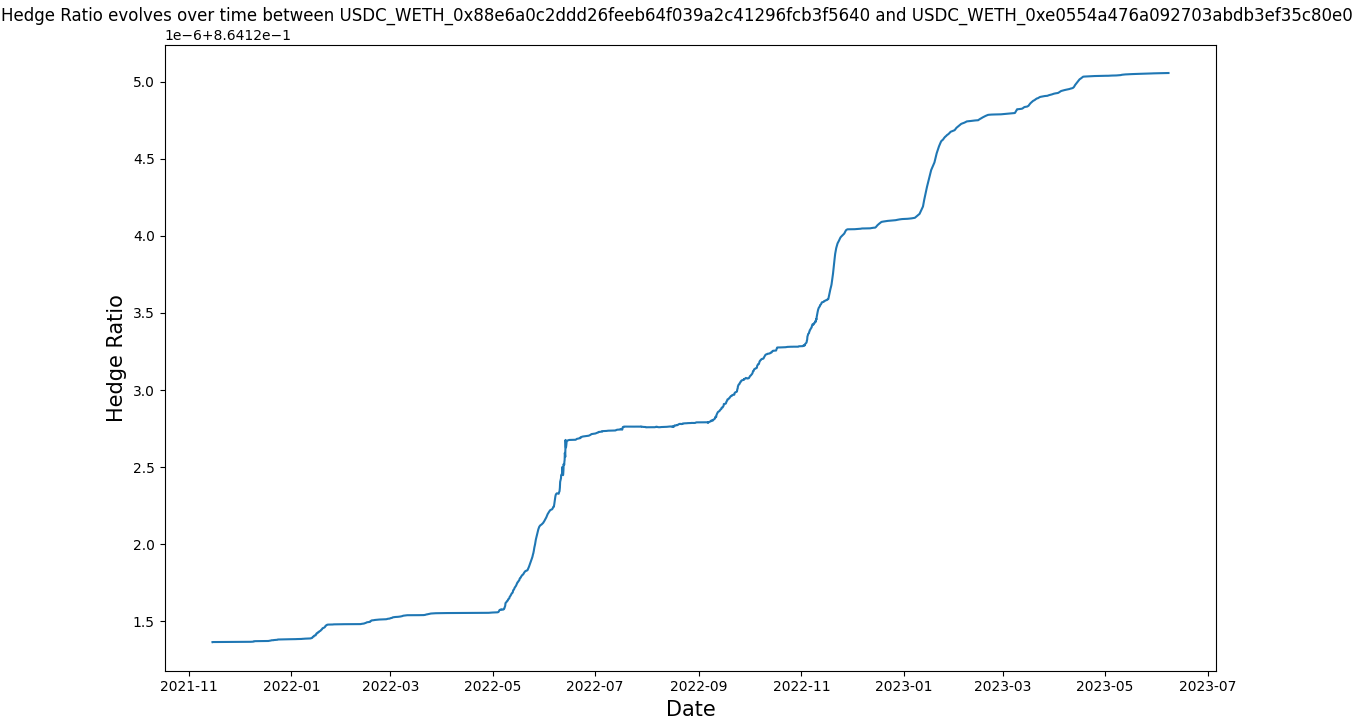
\includegraphics[width=\textwidth]{project/Images/Evolving_hedge_ratio_kf.png}
    \caption{Plot of how the Hedge Ratio using the Kalman Filter \label{fig:evolving_hedge_ratio_kf}}
\end{figure}

\begin{figure}[!htb]
    \centering
    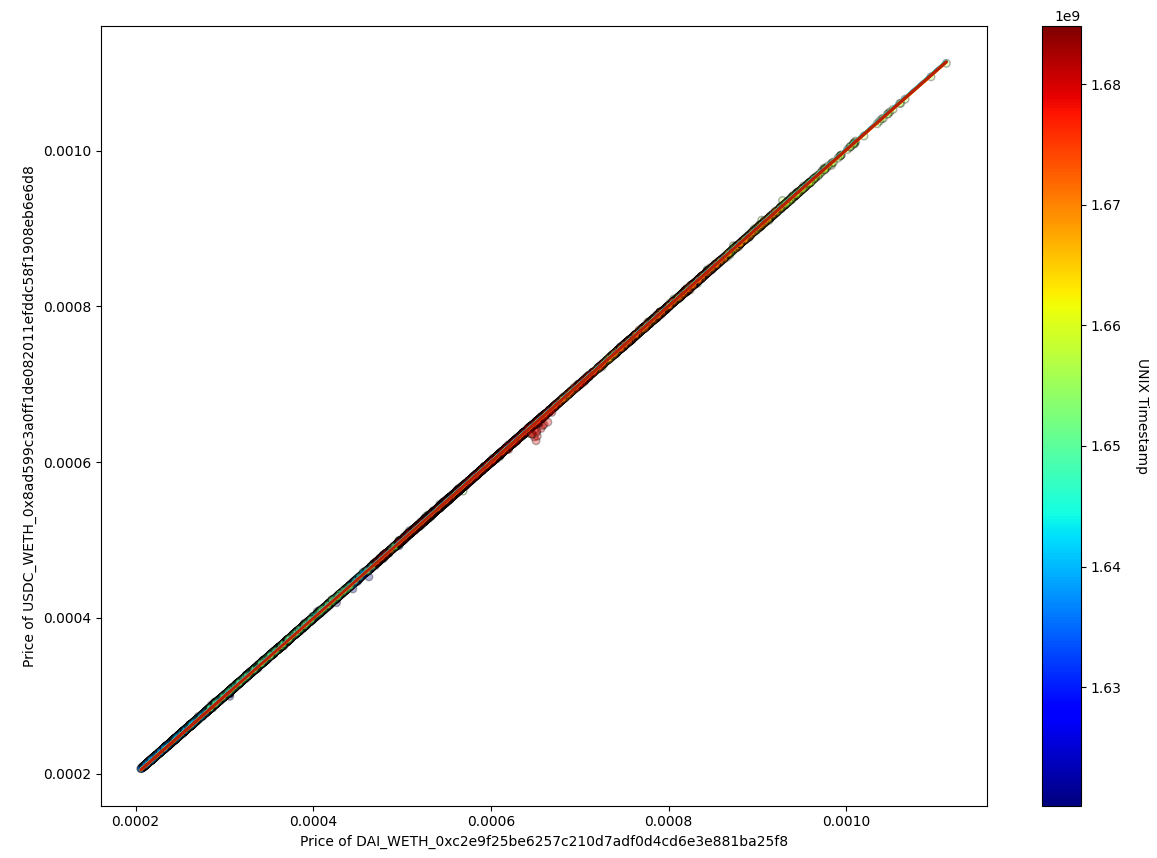
\includegraphics[width=\textwidth]{project/Images/plots_1.png}
    \caption{The plot shows the Kalman Filter estimating the regression line over time, \label{fig:ratios_kf}}
\end{figure}

\subsection{Fees}
As previously mentioned, when engaging in trading activities, there are several fees that are deducted. These fees serve multiple purposes, including compensating the liquidity providers and addressing the potential lack of access to assets from the lender. Therefore, in this section, we will delve into the various costs associated with implementing and executing the strategy.

\subsubsection{Gas Fees}
Gas fees in Ethereum are a crucial component of the network's operation. They serve two main purposes: to prevent spam and denial-of-service attacks and to incentivize miners to include transactions in the blockchain. They are a measure of computational effort required to execute a transaction or perform a smart contract operation on the Ethereum network. Each operation, such as sending tokens, executing a smart contract function, or interacting with decentralized applications, consumes a certain amount of gas.
\\[5mm]
The fee is calculated by multiplying the gas price (expressed in Gwei, where 1 Gwei is equal to 0.000000001 ETH) by the gas used~\cite{noauthor_gas_nodate}. As mentioned in previous sections, when a transaction is initiated by a user, the user specifies the gas limit which defines the maximum amount of gas that a user is willing to pay for a transaction, if the gas limit is too low and the gas used is greater than its limit, the transaction will fail and be reverted. This means that the state changes made by the transaction will not be recorded on Ethereum, and the fees paid for that transaction will be lost.

\begin{figure}[!htb]
    \centering
    \begin{subfigure}[b]{\textwidth}
        \makebox[\textwidth]{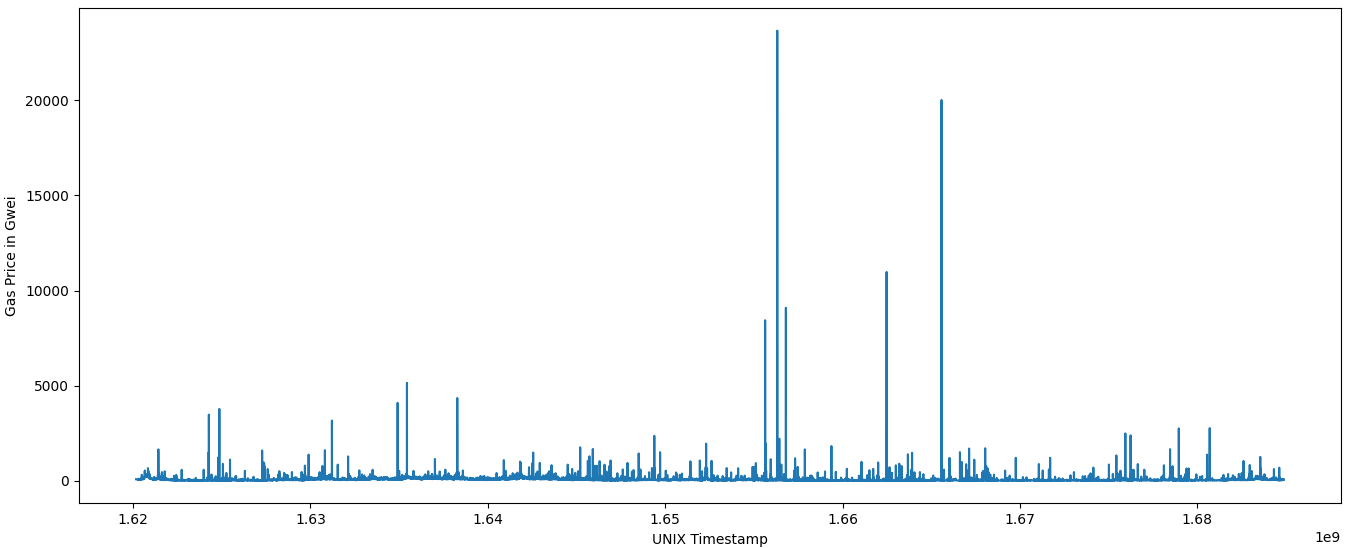
\includegraphics[width=1.15\textwidth]{project/Images/gas_price_1.png}}
    \end{subfigure}
    \hfill
    \begin{subfigure}[b]{\textwidth}
        \centering
        \makebox[\textwidth]{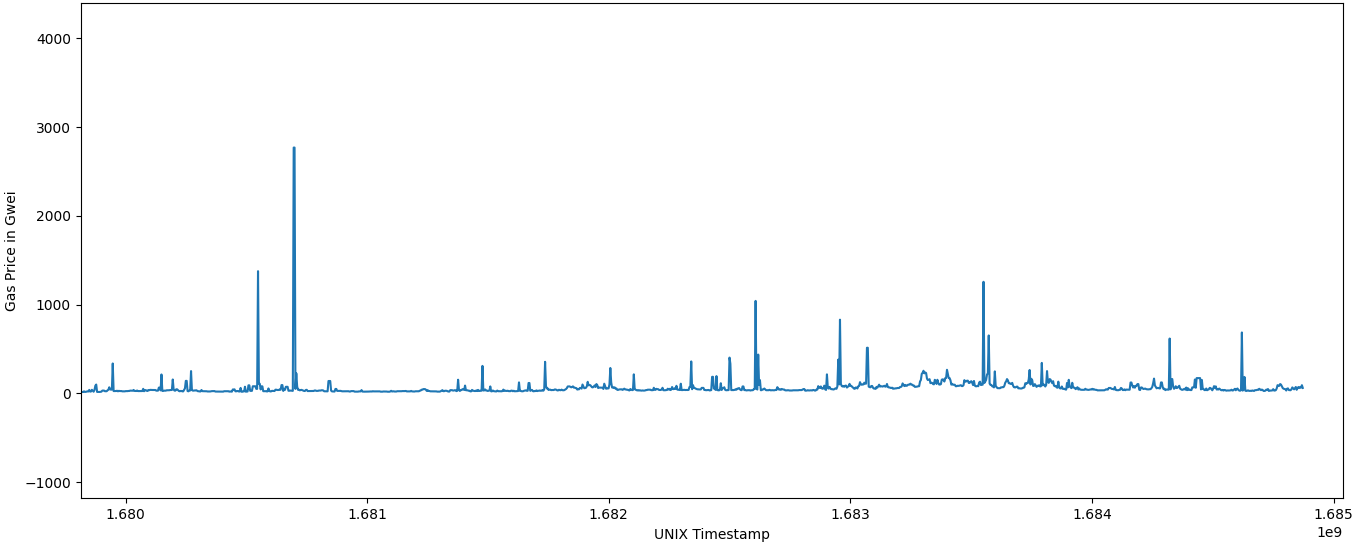
\includegraphics[width=1.15\textwidth]{project/Images/gas_price_2.png}}
    \end{subfigure}
    \vspace{-0.8cm}
    \caption{The top picture shows the gas price over time, while the bottom picture is a zoomed-in plot.}
    \label{fig:gwei_over_time}
\end{figure}

\noindent Figure \ref{fig:gwei_over_time} the gas price history over time, showing the price surges and trophs. The reason for these fluctuations that it is determined by the market forces of supply and demand. It is the amount of Ether (ETH) that a user is willing to pay for each unit of gas consumed in a transaction. Miners have the option to prioritize transactions with higher gas prices, and thus are incentivized to include transactions with higher gas prices because they receive the gas fees as a reward for their mining efforts. Therefore, setting a higher gas price increases the chances of a transaction being executed.
\\[5mm]
The second part of the gas fee is how much gas is used, it is calculated by multiplying the gas cost of each operation in the transaction by the corresponding gas price. Each operation has a predefined gas cost associated with it, which reflects the complexity and resource requirements of that operation. When a transaction or smart contract execution is initiated, the Ethereum Virtual Machine (EVM) processes each operation and deducts the corresponding gas cost from the gas limit. In addition to this, Ethereum also has a base fee with all of their transactions thus having multiple small transaction becomes more costly than using a large combined transaction~\cite{noauthor_gas_nodate}.

\subsubsection{Uniswap Fees}
In addition to transaction fees, there is another fee mechanism in place within the system when swapping on Uniswap. This fee is designed to incentivize and reward liquidity providers on the platform. When a swap occurs, a fee is deducted from the amount of tokens expected to be returned to the user.
\\[5mm]
The fee is calculated as a percentage of the swap volume, meaning that the larger the swap, the higher the fee. For example, let's consider a scenario where the exchange price is 1 TKNA = 100 TKNB and the fee is set at 0.3\%. If someone exchanges 1 TKNA for TKNB, instead of receiving the full 100 TKNB based on the exchange rate, they will receive 100$\times$(1 - 0.3\%) TKNB = 99.7 TKNB. The fee reduces the total amount of tokens received in the swap.
\\[5mm]
It's important to note that the specific fee percentage may vary between different liquidity pools on Uniswap. Each liquidity pool can have its own fee tier, and the fees associated with each interested liquidity pools can be seen in the table below.

\begin{table}[!htb]
    \begin{tabular}{|l|l|l|r|}
        \hline
                                      Pool Address & Token0 & Token1 &  Fee Tier as a \% \\\hline\hline
        0xcbcdf9626bc03e24f779434178a73a0b4bad62ed &   WBTC &   WETH &     0.30 \\\hline
        0xc2e9f25be6257c210d7adf0d4cd6e3e881ba25f8 &    DAI &   WETH &     0.30 \\\hline
        0x8ad599c3a0ff1de082011efddc58f1908eb6e6d8 &   USDC &   WETH &     0.30 \\\hline
        0x4e68ccd3e89f51c3074ca5072bbac773960dfa36 &   WETH &   USDT &     0.30 \\\hline
        0x60594a405d53811d3bc4766596efd80fd545a270 &    DAI &   WETH &     0.05 \\\hline
        0x4585fe77225b41b697c938b018e2ac67ac5a20c0 &   WBTC &   WETH &     0.05 \\\hline
        0x88e6a0c2ddd26feeb64f039a2c41296fcb3f5640 &   USDC &   WETH &     0.05 \\\hline
        0x11b815efb8f581194ae79006d24e0d814b7697f6 &   WETH &   USDT &     0.05 \\\hline
    \end{tabular}
\end{table}

\subsubsection{Aave Fees \& Collatoral}
Aave facilitates lending and borrowing transactions among users, and as part of its operations and incentive mechanisms, it imposes certain fees. In the context of this trading strategy, the only fees applicable would be the interest rates on the loan. The interest rate is typically expressed as an Annual Percentage Yield (APY) and is accrued continuously. Currently, Aave supports variable interest rates, which fluctuate based on market conditions, the borrowed asset, and supply and demand dynamics within the Aave.
\\[5mm]
Another aspect of Aave for the trading strategy is collateralization and the avoidance of liquidation. Liquidation occurs when a borrower's position is forcibly closed, and their collateral assets are sold off in cases of default or insufficient collateral. When borrowing from Aave, borrowers are required to allocate a certain percentage of the loan value as collateral, known as the Loan-to-Value (LTV) ratio~\cite{aave_risk}. For instance, if a token has a 75\% LTV, borrowers can borrow 0.75 ETH worth of the corresponding token for every 1 ETH worth of collateral provided. However, as token prices fluctuate, the ratio between the borrowed token value and the collateral value changes, posing risks for both lenders and Aave. To safeguard lenders and maintain protocol solvency, a liquidation threshold is established. If the collateral value falls below this threshold, the borrower's position becomes vulnerable to liquidation. In such cases, the collateral is auctioned off to repay the outstanding debt to the lenders. Typically, the liquidation threshold is set 5-10\% higher than the asset's LTV. For WETH, the Loan-to-Value ratio is 82.5\%, and the liquidation threshold is 86\%.

\subsection{Overall Strategy}
The implementation of these strategies is intricate, as it is designed to be scalable and highly customizable with various parameters. Additionally, since the strategies being investigated are based on mean reversion, an abstract strategy is created to allow for quick exploration and research into different approaches and the impact of hedge ratio calculations on returns. This abstract strategy encompasses the core logic of generating trading signals, determining optimal trade timing and volumes, and transmitting them to the live or backtesting system. The strategy-specific classes contain operations that calculate the hedge ratio and establish the thresholds that trigger the generation of trading signals. Below shows the functions that the abstract strategy possesses.
\vspace{5mm}
\begin{lstlisting}[language=Python]
class Abstract_Strategy():
    def __init__(self, number_of_sds_from_mean, window_size_in_seconds, percent_to_invest, strategy_name, gas_price_threshold, rebalance_threshold_as_percent_of_initial_investment):
        ...

    def initialise_historical_data(self, history_p1, history_p2):
        ...

    def recalculate_thresholds(self, has_trade=False):
        raise NotImplementedError("recalculate_thresholds not implemented")

    def new_tick(self, price_of_pair1, price_of_pair2, has_trade):
        ...

    def generate_signal(self, ctx, prices):
        ...

\end{lstlisting}
\vspace{5mm}

The functions \texttt{\_\_init\_\_,\ initialise\_historical\_data,\ new\_tick} and \texttt{generate\_signal} are all inheritted by each strategy and \texttt{recalculate\_thresholds} is implemented in each instance of the strategy. \texttt{\_\_init\_\_,\ initialise\_historical\_data} are self explanatory. \texttt{new\_tick} is called in \texttt{generate\_signal} to update the strategy's knowledge of historical prices, this function also triggers a call to \texttt{recalculate\_thresholds} which re-calculates the hedge ratio and determines the thresholds at which an arbitrage opportunity becomes apparent. \texttt{generate\_signal} is the function that is called by the trading system at each price update, it first invokes \texttt{new\_tick} which in turn updates the thresholds, finally the updated hedge ratio and thresholds are used in the process of generating a signal. The steps of \texttt{generate\_signal} are outlined below:
\begin{enumerate}
    \item The first step is to call \texttt{new\_tick} which updates the thresholds
    \item Second, is to check whether a position is already held;
    \begin{enumerate}
        \item If a position IS held, the first is to check if the spread is between the thresholds and if the gas price is below that the specified limit, the positions are closed. Otherwise, the loan to value health factor is calculated, if it may cause liquidation, additional collateral is deposited in Aave.
        \item However, if a position is NOT held and the gas price is below that the specified limit, there are 3 cases. \begin{enumerate}
            \item $spread > upper\_threshold$ - Buy pair 2 and sell pair 1
            \item $spread > lower\_threshold$ - Buy pair 1 and sell pair 2
            \item No trade
        \end{enumerate}
        Furthermore, if a trade is ordered, it is also checked, if the WETH balance falls below the rebalance threshold, the additional tokens are converted back to WETH.
    \end{enumerate}
    In addition, prior to opening or closing a position, a preliminary check is conducted to ensure that the ETH balance remains positive. If the anticipated balance after executing the orders indicates a potential shortfall, an order to \texttt{BUY\ ETH} is automatically initiated. This precautionary measure ensures that the strategy maintains a positive ETH balance and avoids entering into positions that could lead to negative balances.
\end{enumerate}

\subsubsection{Volume of Trades - TODO}

